\ifdefined\beamerclass
\else
    \def\beamerclass{beamer}
\fi
\documentclass[\beamerclass,aspectratio=1610]{beamer}

\usepackage{pgfpages}

\usepackage{biblatex}
\addbibresource{refs.bib}

\usepackage{lmodern}
\usepackage{listings}
\usepackage{amsmath}
\usepackage{bm}
\usepackage{textpos} % package for the positioning

\usepackage{pgf, tikz}
\usepackage{mathdots}
\usepackage{yhmath}
\usepackage{cancel}
\usepackage{color}
\usepackage{siunitx}
\usepackage{array}
\usepackage{multirow}
\usepackage{amssymb}
\usepackage{gensymb}
\usepackage{tabularx}
\usepackage{booktabs}
\usetikzlibrary{fadings}
\usetikzlibrary{arrows, automata}

\setbeamerfont{footnote}{size=\tiny}

\usetheme{Copenhagen}
\hypersetup{pdfstartview={Fit}}
\lstset{basicstyle=\small\ttfamily,breaklines=true}

\title[Learning to Communicate]{Learning to Communicate: Challenges in optimising deep stochastic networks with categorical sampling}
\author{Jonathon Hare}
\institute[]
{
  Vision, Learning and Control\\
  University of Southampton 
}
\date{}
\subject{Computer Science}
\useoutertheme{infolines}
\setbeamertemplate{headline}{} %remove headline
\setbeamertemplate{navigation symbols}{} %remove navigation symbols

\begin{document}
  \frame{
    \titlepage
    \center
    \tiny{The idea for this presentation comes from recent work with my PhD student Daniela Mihai in our upcoming NeurIPS workshop paper: \fullcite{Mihai19}. Some  of the things I'll mention in passing relate to papers with another student, Yan Zhang, and Adam Pr\"ugel-Bennett.}
  }

\begin{frame}
\frametitle{Contents}
\begin{itemize}
	\item Deep Learning 101
	\item Learning to Play Communication Games
	\item What tools do we need to learn such a model?
	\item What do these models learn?
	\item Future Challenges
\end{itemize}
\end{frame}

\begin{frame}{pause}
\frametitle{Machine Learning - A Recap}
{\tiny All credit for this slide goes to Niranjan}\\
\vspace{5mm}
\begin{tabular}{ll}
Data & $\{\bm{x}_n, \bm{y}_n\}^N_{n=1} \qquad \{\bm{x}_n\}^N_{n=1}$ 
\vspace{3mm} \\ 
Function Approximator & $\bm{y} = f (\bm{x}, \bm{\theta}) + \nu$ 
\vspace{3mm} \\ 
Parameter Estimation & $E_0 = \sum^N_{n=1} \{\|\bm{y}_n - f (\bm{x}_n; \bm{\theta})\|\}^2$
\vspace{3mm} \\ 
Prediction & $\bm{\hat y}_{N+1} = f(\bm{x}_{N+1}, \bm{\hat \theta})$
\vspace{3mm} \\ 
Regularisation & $E_1 = \sum^N_{n=1} \{\|\bm{y}_n - f (\bm{x}_n; \bm{\theta})\|\}^2 + r(\|\bm\theta\|)$
\vspace{3mm} \\ 
Modelling Uncertainty & $p(\bm\theta|\{\bm x_n, \bm y_n\}_{n=1}^N)$
\vspace{3mm} \\ 
Probabilistic Inference & $\mathop{\mathbb{E}}[g(\bm\theta)] = \int g(\bm\theta)p(\bm\theta)d\bm\theta = \frac{1}{N_s}\sum_{n=1}^{N_s}g(\bm\theta^{(n)})$
\vspace{3mm} \\ 
Sequence Modelling & $\bm x_n = f(\bm x_{n-1}, \bm\theta)$
\end{tabular}
\vspace{5mm}
\end{frame}

\begin{frame}
\frametitle{What is Deep Learning?}

Deep learning is primarily characterised by large datasets and function compositions with many parameters: \\ \vspace{10mm}
\begin{itemize}
	\item<2-> Feedforward networks: $\bm{y} = f (g(\bm{x}, \bm\theta_g), \bm{\theta_f})$
	\begin{itemize}
		\item Often with relatively simple functions - e.g.:\\
		$f(\bm x, \bm{\theta}_f) = \sigma(\bm{x}^\top \bm{\theta}_f)$ or $f(\bm x, \bm{\theta}_f) = \sigma(\bm{x} \star \bm{\theta}_f)$
	\end{itemize} \vspace{3mm}
	\item<3-> Recurrent networks: $\bm y_t = f(\bm y_{t-1}, \bm x_t, \bm\theta) = f(f(\bm y_{t-2}, \bm x_{t-1}, \bm\theta), \bm\theta) = \dots$
\end{itemize}
\vspace{10mm}

\uncover<4->{
In the early days the focus of deep learning was on learning functions for classification. Nowadays the functions are much more general in their inputs and outputs.
}
\end{frame}

\begin{frame}
\frametitle{A deep learning example: object detection}
\centering
\includegraphics[scale=0.55]{coco2.png}
\end{frame}

\begin{frame}
\frametitle{Differentiable Programming}

\begin{itemize}
	\item Differentiable programming is a term coined by Yann Lecun\footnote{https://www.facebook.com/yann.lecun/posts/10155003011462143} to describe a superset of Deep Learning.
	\item Captures the idea that computer programs can be constructed of parameterised functional blocks in which the parameters are learned using some form of \textbf{gradient-based optimisation.}
	\begin{itemize}
		\item The implication is that we need to be able to compute gradients with respect to the parameters of these functional blocks. 
		\pause
		\item The idea of Differentiable Programming also opens up interesting possibilities: 
		\begin{itemize}
			\item The functional blocks don't need to be direct functions in a mathematical sense; more generally they can be \emph{algorithms}.
			\item What if the functional block we're learning parameters for is itself an algorithm that optimises the parameters of an internal algorithm using a gradient based optimiser?!\footfullcite{zhang2018learning}\textsuperscript{,}\footfullcite{zhang2019dspn}
		\end{itemize}
	\end{itemize}
\end{itemize}
\end{frame}

\begin{frame}
\frametitle{Learning to Play Communication Games: Motivation}

\begin{itemize}
	\item As humans, our understanding and conceptualisation of the visual world is very much linked with our ability to communicate using natural language.
	\item Machine learners (and mathematicians) have long understood that forcing data through a bottleneck can lead to representations that capture information.
	\item \textbf{We want to explore if a `language bottleneck' between a pair of agents performing collaborative tasks can encourage the emergence of a communication protocol that captures visual semantics.}
	\begin{itemize}	
		\item We'll assume a `language bottleneck' means a variable length sequence of discrete tokens drawn from a fixed size vocabulary.
	\end{itemize}
\end{itemize}

\end{frame}

\begin{frame}
\frametitle{A Referential Communication Game}

\begin{figure}
\centering
\includegraphics[width=0.7\textwidth]{game.png}	
\end{figure}

A Referential Game\footfullcite{Lewis1969-LEWCAP-4}: Alice must communicate to Bob which image she has (Bob has that image, plus many distractors). Communication is one-way only. Alice knows nothing about the distractors Bob has (they could all be white boats!).
\end{frame}

\begin{frame}
\frametitle{A Computational Model}
This is the model proposed by \citeauthor{Havrylov2017}\footfullcite{Havrylov2017}:
\begin{figure}
    \centering
    \resizebox{0.7\textwidth}{!}{

\tikzset{every picture/.style={line width=0.75pt}} %set default line width to 0.75pt        

\begin{tikzpicture}[x=0.75pt,y=0.75pt,yscale=-1,xscale=1]
%uncomment if require: \path (0,346); %set diagram left start at 0, and has height of 346

%Shape: Rectangle [id:dp047937671636080315] 
\draw  [fill={rgb, 255:red, 126; green, 211; blue, 33 }  ,fill opacity=1 ] (235,80.2) -- (245,80.2) -- (245,120.2) -- (235,120.2) -- cycle ;
%Shape: Rectangle [id:dp5065635721092933] 
\draw  [fill={rgb, 255:red, 126; green, 211; blue, 33 }  ,fill opacity=1 ] (285,80.2) -- (295,80.2) -- (295,120.2) -- (285,120.2) -- cycle ;
%Shape: Rectangle [id:dp6510643084661036] 
\draw  [fill={rgb, 255:red, 126; green, 211; blue, 33 }  ,fill opacity=1 ] (335,80.2) -- (345,80.2) -- (345,120.2) -- (335,120.2) -- cycle ;
%Shape: Rectangle [id:dp5217874121144922] 
\draw  [fill={rgb, 255:red, 126; green, 211; blue, 33 }  ,fill opacity=1 ] (385,80.2) -- (395,80.2) -- (395,120.2) -- (385,120.2) -- cycle ;
%Shape: Rectangle [id:dp0592658032150114] 
\draw  [fill={rgb, 255:red, 126; green, 211; blue, 33 }  ,fill opacity=1 ] (435,80.2) -- (445,80.2) -- (445,120.2) -- (435,120.2) -- cycle ;
%Shape: Rectangle [id:dp7992522747750251] 
\draw  [fill={rgb, 255:red, 74; green, 144; blue, 226 }  ,fill opacity=1 ] (235,230.2) -- (245,230.2) -- (245,270.2) -- (235,270.2) -- cycle ;
%Shape: Rectangle [id:dp014632675898352931] 
\draw  [fill={rgb, 255:red, 74; green, 144; blue, 226 }  ,fill opacity=1 ] (285,230.2) -- (295,230.2) -- (295,270.2) -- (285,270.2) -- cycle ;
%Shape: Rectangle [id:dp9211786132147152] 
\draw  [fill={rgb, 255:red, 74; green, 144; blue, 226 }  ,fill opacity=1 ] (335,230.2) -- (345,230.2) -- (345,270.2) -- (335,270.2) -- cycle ;
%Shape: Rectangle [id:dp49165732728118716] 
\draw  [fill={rgb, 255:red, 74; green, 144; blue, 226 }  ,fill opacity=1 ] (385,230.2) -- (395,230.2) -- (395,270.2) -- (385,270.2) -- cycle ;
%Shape: Rectangle [id:dp5182365233474338] 
\draw  [fill={rgb, 255:red, 74; green, 144; blue, 226 }  ,fill opacity=1 ] (435,230.2) -- (445,230.2) -- (445,270.2) -- (435,270.2) -- cycle ;
%Shape: Rectangle [id:dp26764493526594846] 
\draw  [fill={rgb, 255:red, 74; green, 144; blue, 226 }  ,fill opacity=1 ] (185,230.2) -- (195,230.2) -- (195,270.2) -- (185,270.2) -- cycle ;
%Shape: Rectangle [id:dp617302198114965] 
\draw  [fill={rgb, 255:red, 208; green, 2; blue, 27 }  ,fill opacity=1 ] (235,140) -- (245,140) -- (245,150) -- (235,150) -- cycle ;
%Shape: Rectangle [id:dp07186998587808935] 
\draw  [fill={rgb, 255:red, 208; green, 2; blue, 27 }  ,fill opacity=1 ] (335,140) -- (345,140) -- (345,150) -- (335,150) -- cycle ;
%Shape: Rectangle [id:dp589447034842384] 
\draw  [fill={rgb, 255:red, 208; green, 2; blue, 27 }  ,fill opacity=1 ] (285,140) -- (295,140) -- (295,150) -- (285,150) -- cycle ;
%Shape: Rectangle [id:dp21595389024935918] 
\draw  [fill={rgb, 255:red, 208; green, 2; blue, 27 }  ,fill opacity=1 ] (385,140.2) -- (395,140.2) -- (395,150.2) -- (385,150.2) -- cycle ;
%Shape: Rectangle [id:dp0802795080857045] 
\draw  [fill={rgb, 255:red, 208; green, 2; blue, 27 }  ,fill opacity=1 ] (435,140) -- (445,140) -- (445,150) -- (435,150) -- cycle ;
%Shape: Rectangle [id:dp8232915052139519] 
\draw  [fill={rgb, 255:red, 245; green, 166; blue, 35 }  ,fill opacity=1 ] (235,175) -- (245,175) -- (245,185) -- (235,185) -- cycle ;
%Shape: Rectangle [id:dp16034237925020733] 
\draw  [fill={rgb, 255:red, 245; green, 166; blue, 35 }  ,fill opacity=1 ] (335,175) -- (345,175) -- (345,185) -- (335,185) -- cycle ;
%Shape: Rectangle [id:dp30877673380837534] 
\draw  [fill={rgb, 255:red, 245; green, 166; blue, 35 }  ,fill opacity=1 ] (285,175) -- (295,175) -- (295,185) -- (285,185) -- cycle ;
%Shape: Rectangle [id:dp4068155165804904] 
\draw  [fill={rgb, 255:red, 245; green, 166; blue, 35 }  ,fill opacity=1 ] (385,175) -- (395,175) -- (395,185) -- (385,185) -- cycle ;
%Shape: Rectangle [id:dp5507673779424204] 
\draw  [fill={rgb, 255:red, 245; green, 166; blue, 35 }  ,fill opacity=1 ] (435,175) -- (445,175) -- (445,185) -- (435,185) -- cycle ;
%Shape: Rectangle [id:dp3639162773569877] 
\draw  [fill={rgb, 255:red, 189; green, 16; blue, 224 }  ,fill opacity=1 ] (235,290.2) -- (245,290.2) -- (245,300.2) -- (235,300.2) -- cycle ;
%Shape: Rectangle [id:dp557317243000601] 
\draw  [fill={rgb, 255:red, 189; green, 16; blue, 224 }  ,fill opacity=1 ] (335,290.2) -- (345,290.2) -- (345,300.2) -- (335,300.2) -- cycle ;
%Shape: Rectangle [id:dp18867874640873628] 
\draw  [fill={rgb, 255:red, 189; green, 16; blue, 224 }  ,fill opacity=1 ] (285,290.2) -- (295,290.2) -- (295,300.2) -- (285,300.2) -- cycle ;
%Shape: Rectangle [id:dp5219403278372264] 
\draw  [fill={rgb, 255:red, 189; green, 16; blue, 224 }  ,fill opacity=1 ] (385,290.2) -- (395,290.2) -- (395,300.2) -- (385,300.2) -- cycle ;
%Shape: Rectangle [id:dp13430408666216642] 
\draw  [fill={rgb, 255:red, 189; green, 16; blue, 224 }  ,fill opacity=1 ] (435,290.2) -- (445,290.2) -- (445,300.2) -- (435,300.2) -- cycle ;
%Straight Lines [id:da5932739256293282] 
\draw    (195,250.2) -- (233,250.2) ;
\draw [shift={(235,250.2)}, rotate = 180] [fill={rgb, 255:red, 0; green, 0; blue, 0 }  ][line width=0.75]  [draw opacity=0] (8.93,-4.29) -- (0,0) -- (8.93,4.29) -- cycle    ;

%Straight Lines [id:da06455409369010945] 
\draw    (245,250.2) -- (283,250.2) ;
\draw [shift={(285,250.2)}, rotate = 180] [fill={rgb, 255:red, 0; green, 0; blue, 0 }  ][line width=0.75]  [draw opacity=0] (8.93,-4.29) -- (0,0) -- (8.93,4.29) -- cycle    ;

%Straight Lines [id:da7219957398344385] 
\draw    (295,250.2) -- (333,250.2) ;
\draw [shift={(335,250.2)}, rotate = 180] [fill={rgb, 255:red, 0; green, 0; blue, 0 }  ][line width=0.75]  [draw opacity=0] (8.93,-4.29) -- (0,0) -- (8.93,4.29) -- cycle    ;

%Straight Lines [id:da43994896820081186] 
\draw    (345,250.2) -- (383,250.2) ;
\draw [shift={(385,250.2)}, rotate = 180] [fill={rgb, 255:red, 0; green, 0; blue, 0 }  ][line width=0.75]  [draw opacity=0] (8.93,-4.29) -- (0,0) -- (8.93,4.29) -- cycle    ;

%Straight Lines [id:da44487946410609513] 
\draw    (395,250.2) -- (433,250.2) ;
\draw [shift={(435,250.2)}, rotate = 180] [fill={rgb, 255:red, 0; green, 0; blue, 0 }  ][line width=0.75]  [draw opacity=0] (8.93,-4.29) -- (0,0) -- (8.93,4.29) -- cycle    ;

%Straight Lines [id:da48812303680334335] 
\draw    (240,290.2) -- (240,272.2) ;
\draw [shift={(240,270.2)}, rotate = 450] [fill={rgb, 255:red, 0; green, 0; blue, 0 }  ][line width=0.75]  [draw opacity=0] (8.93,-4.29) -- (0,0) -- (8.93,4.29) -- cycle    ;

%Straight Lines [id:da29440027821819326] 
\draw    (290,290.2) -- (290,272.2) ;
\draw [shift={(290,270.2)}, rotate = 450] [fill={rgb, 255:red, 0; green, 0; blue, 0 }  ][line width=0.75]  [draw opacity=0] (8.93,-4.29) -- (0,0) -- (8.93,4.29) -- cycle    ;

%Straight Lines [id:da5047232820516745] 
\draw    (340,290.2) -- (340,272.2) ;
\draw [shift={(340,270.2)}, rotate = 450] [fill={rgb, 255:red, 0; green, 0; blue, 0 }  ][line width=0.75]  [draw opacity=0] (8.93,-4.29) -- (0,0) -- (8.93,4.29) -- cycle    ;

%Straight Lines [id:da9217561800792564] 
\draw    (390,290.2) -- (390,272.2) ;
\draw [shift={(390,270.2)}, rotate = 450] [fill={rgb, 255:red, 0; green, 0; blue, 0 }  ][line width=0.75]  [draw opacity=0] (8.93,-4.29) -- (0,0) -- (8.93,4.29) -- cycle    ;

%Straight Lines [id:da5732345004570589] 
\draw    (440,290.2) -- (440,272.2) ;
\draw [shift={(440,270.2)}, rotate = 450] [fill={rgb, 255:red, 0; green, 0; blue, 0 }  ][line width=0.75]  [draw opacity=0] (8.93,-4.29) -- (0,0) -- (8.93,4.29) -- cycle    ;

%Straight Lines [id:da53216217109383] 
\draw    (240,175) -- (240,152) ;
\draw [shift={(240,150)}, rotate = 450] [fill={rgb, 255:red, 0; green, 0; blue, 0 }  ][line width=0.75]  [draw opacity=0] (8.93,-4.29) -- (0,0) -- (8.93,4.29) -- cycle    ;

%Straight Lines [id:da8976174404653392] 
\draw    (240,140.2) -- (240,122.2) ;
\draw [shift={(240,120.2)}, rotate = 450] [fill={rgb, 255:red, 0; green, 0; blue, 0 }  ][line width=0.75]  [draw opacity=0] (8.93,-4.29) -- (0,0) -- (8.93,4.29) -- cycle    ;

%Straight Lines [id:da715232656071301] 
\draw    (290,175) -- (290,152.2) ;
\draw [shift={(290,150.2)}, rotate = 450] [fill={rgb, 255:red, 0; green, 0; blue, 0 }  ][line width=0.75]  [draw opacity=0] (8.93,-4.29) -- (0,0) -- (8.93,4.29) -- cycle    ;

%Straight Lines [id:da9499056062493815] 
\draw    (290,140.2) -- (290,122.2) ;
\draw [shift={(290,120.2)}, rotate = 450] [fill={rgb, 255:red, 0; green, 0; blue, 0 }  ][line width=0.75]  [draw opacity=0] (8.93,-4.29) -- (0,0) -- (8.93,4.29) -- cycle    ;

%Straight Lines [id:da4170655626870391] 
\draw    (340,175) -- (340,152.2) ;
\draw [shift={(340,150.2)}, rotate = 450] [fill={rgb, 255:red, 0; green, 0; blue, 0 }  ][line width=0.75]  [draw opacity=0] (8.93,-4.29) -- (0,0) -- (8.93,4.29) -- cycle    ;

%Straight Lines [id:da10349432320464413] 
\draw    (340,140.2) -- (340,122.2) ;
\draw [shift={(340,120.2)}, rotate = 450] [fill={rgb, 255:red, 0; green, 0; blue, 0 }  ][line width=0.75]  [draw opacity=0] (8.93,-4.29) -- (0,0) -- (8.93,4.29) -- cycle    ;

%Straight Lines [id:da019316792347473744] 
\draw    (390,175) -- (390,152.2) ;
\draw [shift={(390,150.2)}, rotate = 450] [fill={rgb, 255:red, 0; green, 0; blue, 0 }  ][line width=0.75]  [draw opacity=0] (8.93,-4.29) -- (0,0) -- (8.93,4.29) -- cycle    ;

%Straight Lines [id:da5307347180106695] 
\draw    (390,140) -- (390,122) ;
\draw [shift={(390,120)}, rotate = 450] [fill={rgb, 255:red, 0; green, 0; blue, 0 }  ][line width=0.75]  [draw opacity=0] (8.93,-4.29) -- (0,0) -- (8.93,4.29) -- cycle    ;

%Straight Lines [id:da259343024354849] 
\draw    (440,175) -- (440,152.2) ;
\draw [shift={(440,150.2)}, rotate = 450] [fill={rgb, 255:red, 0; green, 0; blue, 0 }  ][line width=0.75]  [draw opacity=0] (8.93,-4.29) -- (0,0) -- (8.93,4.29) -- cycle    ;

%Straight Lines [id:da8912156912727136] 
\draw    (440,140.2) -- (440,122.2) ;
\draw [shift={(440,120.2)}, rotate = 450] [fill={rgb, 255:red, 0; green, 0; blue, 0 }  ][line width=0.75]  [draw opacity=0] (8.93,-4.29) -- (0,0) -- (8.93,4.29) -- cycle    ;

%Straight Lines [id:da4221172691884344] 
\draw    (245,100.2) -- (283,100.2) ;
\draw [shift={(285,100.2)}, rotate = 180] [fill={rgb, 255:red, 0; green, 0; blue, 0 }  ][line width=0.75]  [draw opacity=0] (8.93,-4.29) -- (0,0) -- (8.93,4.29) -- cycle    ;

%Straight Lines [id:da35786348178728045] 
\draw    (295,100.2) -- (333,100.2) ;
\draw [shift={(335,100.2)}, rotate = 180] [fill={rgb, 255:red, 0; green, 0; blue, 0 }  ][line width=0.75]  [draw opacity=0] (8.93,-4.29) -- (0,0) -- (8.93,4.29) -- cycle    ;

%Straight Lines [id:da15828333576421816] 
\draw    (345,100.2) -- (383,100.2) ;
\draw [shift={(385,100.2)}, rotate = 180] [fill={rgb, 255:red, 0; green, 0; blue, 0 }  ][line width=0.75]  [draw opacity=0] (8.93,-4.29) -- (0,0) -- (8.93,4.29) -- cycle    ;

%Straight Lines [id:da3286319932944599] 
\draw    (395,100.2) -- (433,100.2) ;
\draw [shift={(435,100.2)}, rotate = 180] [fill={rgb, 255:red, 0; green, 0; blue, 0 }  ][line width=0.75]  [draw opacity=0] (8.93,-4.29) -- (0,0) -- (8.93,4.29) -- cycle    ;

%Straight Lines [id:da9724267446103516] 
\draw    (240,230.2) -- (240,190) ;
\draw [shift={(240,190)}, rotate = 450] [color={rgb, 255:red, 0; green, 0; blue, 0 }  ][line width=0.75]    (0,5.59) -- (0,-5.59)   ;

%Straight Lines [id:da1815483054750766] 
\draw    (290,230.2) -- (290,190) ;
\draw [shift={(290,190)}, rotate = 450] [color={rgb, 255:red, 0; green, 0; blue, 0 }  ][line width=0.75]    (0,5.59) -- (0,-5.59)   ;

%Straight Lines [id:da6492306358383702] 
\draw    (340,230.2) -- (340,190) ;
\draw [shift={(340,190)}, rotate = 450] [color={rgb, 255:red, 0; green, 0; blue, 0 }  ][line width=0.75]    (0,5.59) -- (0,-5.59)   ;

%Straight Lines [id:da9814210106657848] 
\draw    (390,230.2) -- (390,190) ;
\draw [shift={(390,190)}, rotate = 450] [color={rgb, 255:red, 0; green, 0; blue, 0 }  ][line width=0.75]    (0,5.59) -- (0,-5.59)   ;

%Straight Lines [id:da803960259370653] 
\draw    (440,230.2) -- (440,190) ;
\draw [shift={(440,190)}, rotate = 450] [color={rgb, 255:red, 0; green, 0; blue, 0 }  ][line width=0.75]    (0,5.59) -- (0,-5.59)   ;

%Flowchart: Manual Operation [id:dp18158503449085273] 
\draw  [fill={rgb, 255:red, 248; green, 231; blue, 28 }  ,fill opacity=1 ] (560,144.38) -- (590,135) -- (590,185) -- (560,175.63) -- cycle ;
%Flowchart: Manual Operation [id:dp5360532561106421] 
\draw  [fill={rgb, 255:red, 248; green, 231; blue, 28 }  ,fill opacity=1 ] (560,84.38) -- (590,75) -- (590,125) -- (560,115.63) -- cycle ;
%Flowchart: Manual Operation [id:dp8939253642889028] 
\draw  [fill={rgb, 255:red, 248; green, 231; blue, 28 }  ,fill opacity=1 ] (560,24.38) -- (590,15) -- (590,65) -- (560,55.63) -- cycle ;
%Flowchart: Manual Operation [id:dp16207172533550307] 
\draw  [fill={rgb, 255:red, 248; green, 231; blue, 28 }  ,fill opacity=1 ] (110.06,265.81) -- (80,275) -- (80.3,225) -- (110.25,234.56) -- cycle ;
%Shape: Rectangle [id:dp3366695110332466] 
\draw  [fill={rgb, 255:red, 139; green, 87; blue, 42 }  ,fill opacity=1 ] (135,270.06) -- (125,270) -- (125.24,230) -- (135.24,230.06) -- cycle ;
%Straight Lines [id:da3710002004001587] 
\draw    (160,250) -- (183,250) ;
\draw [shift={(185,250)}, rotate = 180] [fill={rgb, 255:red, 0; green, 0; blue, 0 }  ][line width=0.75]  [draw opacity=0] (8.93,-4.29) -- (0,0) -- (8.93,4.29) -- cycle    ;

%Straight Lines [id:da6055871303293606] 
\draw    (110,249.8) -- (123,249.97) ;
\draw [shift={(125,250)}, rotate = 180.76] [fill={rgb, 255:red, 0; green, 0; blue, 0 }  ][line width=0.75]  [draw opacity=0] (8.93,-4.29) -- (0,0) -- (8.93,4.29) -- cycle    ;

%Straight Lines [id:da9666420272998885] 
\draw    (55,249.8) -- (78,249.8) ;
\draw [shift={(80,249.8)}, rotate = 180] [fill={rgb, 255:red, 0; green, 0; blue, 0 }  ][line width=0.75]  [draw opacity=0] (8.93,-4.29) -- (0,0) -- (8.93,4.29) -- cycle    ;

%Straight Lines [id:da3609128733470398] 
\draw    (605,40) -- (592,40) ;
\draw [shift={(590,40)}, rotate = 360] [fill={rgb, 255:red, 0; green, 0; blue, 0 }  ][line width=0.75]  [draw opacity=0] (8.93,-4.29) -- (0,0) -- (8.93,4.29) -- cycle    ;

%Straight Lines [id:da9602440739620383] 
\draw    (605,100) -- (592,100) ;
\draw [shift={(590,100)}, rotate = 360] [fill={rgb, 255:red, 0; green, 0; blue, 0 }  ][line width=0.75]  [draw opacity=0] (8.93,-4.29) -- (0,0) -- (8.93,4.29) -- cycle    ;

%Straight Lines [id:da40300913500921476] 
\draw    (605,160) -- (592,160) ;
\draw [shift={(590,160)}, rotate = 360] [fill={rgb, 255:red, 0; green, 0; blue, 0 }  ][line width=0.75]  [draw opacity=0] (8.93,-4.29) -- (0,0) -- (8.93,4.29) -- cycle    ;

%Straight Lines [id:da04548317080652242] 
\draw    (560,160) -- (547,160) ;
\draw [shift={(545,160)}, rotate = 360] [fill={rgb, 255:red, 0; green, 0; blue, 0 }  ][line width=0.75]  [draw opacity=0] (8.93,-4.29) -- (0,0) -- (8.93,4.29) -- cycle    ;

%Straight Lines [id:da29875700106160963] 
\draw    (560,100) -- (547,100) ;
\draw [shift={(545,100)}, rotate = 360] [fill={rgb, 255:red, 0; green, 0; blue, 0 }  ][line width=0.75]  [draw opacity=0] (8.93,-4.29) -- (0,0) -- (8.93,4.29) -- cycle    ;

%Straight Lines [id:da37536468051409433] 
\draw    (560,40) -- (547,40) ;
\draw [shift={(545,40)}, rotate = 360] [fill={rgb, 255:red, 0; green, 0; blue, 0 }  ][line width=0.75]  [draw opacity=0] (8.93,-4.29) -- (0,0) -- (8.93,4.29) -- cycle    ;

%Shape: Circle [id:dp009001411304518703] 
\draw   (545,40) .. controls (545,37.24) and (542.76,35) .. (540,35) .. controls (537.24,35) and (535,37.24) .. (535,40) .. controls (535,42.76) and (537.24,45) .. (540,45) .. controls (542.76,45) and (545,42.76) .. (545,40) -- cycle ;
%Shape: Circle [id:dp8025414183464545] 
\draw   (545,100) .. controls (545,97.24) and (542.76,95) .. (540,95) .. controls (537.24,95) and (535,97.24) .. (535,100) .. controls (535,102.76) and (537.24,105) .. (540,105) .. controls (542.76,105) and (545,102.76) .. (545,100) -- cycle ;
%Shape: Circle [id:dp7442495986243576] 
\draw   (545,160) .. controls (545,157.24) and (542.76,155) .. (540,155) .. controls (537.24,155) and (535,157.24) .. (535,160) .. controls (535,162.76) and (537.24,165) .. (540,165) .. controls (542.76,165) and (545,162.76) .. (545,160) -- cycle ;
%Curve Lines [id:da6423332622875322] 
\draw    (499.88,100.03) .. controls (528.44,100.03) and (499.88,42.43) .. (533.42,40.07) ;
\draw [shift={(535,40)}, rotate = 538.94] [fill={rgb, 255:red, 0; green, 0; blue, 0 }  ][line width=0.75]  [draw opacity=0] (8.93,-4.29) -- (0,0) -- (8.93,4.29) -- cycle    ;

%Curve Lines [id:da7303118741492726] 
\draw    (499.88,100.03) .. controls (528.44,100.03) and (499.88,158.86) .. (533.42,159.99) ;
\draw [shift={(535,160)}, rotate = 538.94] [fill={rgb, 255:red, 0; green, 0; blue, 0 }  ][line width=0.75]  [draw opacity=0] (8.93,-4.29) -- (0,0) -- (8.93,4.29) -- cycle    ;

%Straight Lines [id:da10989832498374075] 
\draw    (499.88,100.03) -- (533,100) ;
\draw [shift={(535,100)}, rotate = 539.95] [fill={rgb, 255:red, 0; green, 0; blue, 0 }  ][line width=0.75]  [draw opacity=0] (8.93,-4.29) -- (0,0) -- (8.93,4.29) -- cycle    ;

%Shape: Rectangle [id:dp6112922056074307] 
\draw  [color={rgb, 255:red, 155; green, 155; blue, 155 }  ,draw opacity=1 ] (0,165) -- (450,165) -- (450,335) -- (0,335) -- cycle ;
%Straight Lines [id:da6868285828448821] 
\draw    (445,100) -- (463,100) ;
\draw [shift={(465,100)}, rotate = 180] [fill={rgb, 255:red, 0; green, 0; blue, 0 }  ][line width=0.75]  [draw opacity=0] (8.93,-4.29) -- (0,0) -- (8.93,4.29) -- cycle    ;

%Shape: Rectangle [id:dp16788170272941716] 
\draw  [fill={rgb, 255:red, 80; green, 227; blue, 194 }  ,fill opacity=1 ] (159.76,270.06) -- (149.76,270) -- (150,230) -- (160,230.06) -- cycle ;
%Straight Lines [id:da5281163918010228] 
\draw    (135.15,250.37) -- (148,250.05) ;
\draw [shift={(150,250)}, rotate = 538.5799999999999] [fill={rgb, 255:red, 0; green, 0; blue, 0 }  ][line width=0.75]  [draw opacity=0] (8.93,-4.29) -- (0,0) -- (8.93,4.29) -- cycle    ;

%Shape: Rectangle [id:dp18684504023002002] 
\draw  [color={rgb, 255:red, 155; green, 155; blue, 155 }  ,draw opacity=1 ] (175,10) -- (660,10) -- (660,205) -- (175,205) -- cycle ;
%Image [id:dp06842157057734388] 
\draw (35.15,249.85) node  {\includegraphics[width=37.27pt,height=37.73pt]{automobile4.png}};
%Image [id:dp4120261120891594] 
\draw (629.85,160.15) node  {\includegraphics[width=37.27pt,height=37.73pt]{automobile4.png}};
%Image [id:dp5944420903219944] 
\draw (630,40) node  {\includegraphics[width=37.5pt,height=37.5pt]{horse5.png}};
%Image [id:dp27455499166532515] 
\draw (630,100) node  {\includegraphics[width=37.5pt,height=37.5pt]{ship1.png}};
%Straight Lines [id:da7071120892947695] 
\draw    (240,320) -- (240,302) ;
\draw [shift={(240,300)}, rotate = 450] [fill={rgb, 255:red, 0; green, 0; blue, 0 }  ][line width=0.75]  [draw opacity=0] (8.93,-4.29) -- (0,0) -- (8.93,4.29) -- cycle    ;

%Curve Lines [id:da3166116446927084] 
\draw  [dash pattern={on 0.84pt off 2.51pt}]  (245,180) .. controls (250.01,180.25) and (260.41,179.45) .. (260,245) .. controls (259.6,309.56) and (289.74,341.24) .. (290.01,302.04) ;
\draw [shift={(290,300.2)}, rotate = 449.09] [fill={rgb, 255:red, 0; green, 0; blue, 0 }  ][line width=0.75]  [draw opacity=0] (8.93,-4.29) -- (0,0) -- (8.93,4.29) -- cycle    ;

%Curve Lines [id:da23186178998551776] 
\draw  [dash pattern={on 0.84pt off 2.51pt}]  (295,180) .. controls (300.01,180.25) and (310.41,179.45) .. (310,245) .. controls (309.6,309.56) and (339.74,341.24) .. (340.01,302.04) ;
\draw [shift={(340,300.2)}, rotate = 449.09] [fill={rgb, 255:red, 0; green, 0; blue, 0 }  ][line width=0.75]  [draw opacity=0] (8.93,-4.29) -- (0,0) -- (8.93,4.29) -- cycle    ;

%Curve Lines [id:da07784246562522934] 
\draw  [dash pattern={on 0.84pt off 2.51pt}]  (345,180) .. controls (350.01,180.25) and (360.41,179.45) .. (360,245) .. controls (359.6,309.56) and (389.74,341.24) .. (390.01,302.04) ;
\draw [shift={(390,300.2)}, rotate = 449.09] [fill={rgb, 255:red, 0; green, 0; blue, 0 }  ][line width=0.75]  [draw opacity=0] (8.93,-4.29) -- (0,0) -- (8.93,4.29) -- cycle    ;

%Curve Lines [id:da46243466060506067] 
\draw  [dash pattern={on 0.84pt off 2.51pt}]  (395,180) .. controls (400.01,180.25) and (410.41,179.45) .. (410,245) .. controls (409.6,309.56) and (439.74,341.24) .. (440.01,302.04) ;
\draw [shift={(440,300.2)}, rotate = 449.09] [fill={rgb, 255:red, 0; green, 0; blue, 0 }  ][line width=0.75]  [draw opacity=0] (8.93,-4.29) -- (0,0) -- (8.93,4.29) -- cycle    ;

%Shape: Rectangle [id:dp2500898350294596] 
\draw  [fill={rgb, 255:red, 184; green, 233; blue, 134 }  ,fill opacity=1 ] (474.76,120.06) -- (464.76,120) -- (465,80) -- (475,80.06) -- cycle ;
%Straight Lines [id:da7180400848603097] 
\draw    (475,100) -- (493,100) ;
\draw [shift={(495,100)}, rotate = 180] [fill={rgb, 255:red, 0; green, 0; blue, 0 }  ][line width=0.75]  [draw opacity=0] (8.93,-4.29) -- (0,0) -- (8.93,4.29) -- cycle    ;

%Shape: Rectangle [id:dp3192915442850023] 
\draw  [fill={rgb, 255:red, 82; green, 2; blue, 208 }  ,fill opacity=1 ] (494.88,80.03) -- (504.88,80.03) -- (504.88,120.03) -- (494.88,120.03) -- cycle ;

% Text Node
\draw (224,77.7) node  [align=left] {$\displaystyle h^{r}_{1}$};
% Text Node
\draw (274,77.5) node  [align=left] {$\displaystyle h^{r}_{2}$};
% Text Node
\draw (324,77.7) node  [align=left] {$\displaystyle h^{r}_{3}$};
% Text Node
\draw (374,77.7) node  [align=left] {$\displaystyle h^{r}_{4}$};
% Text Node
\draw (424,77.7) node  [align=left] {$\displaystyle h^{r}_{5}$};
% Text Node
\draw (224,227.5) node  [align=left] {$\displaystyle h^{s}_{1}$};
% Text Node
\draw (274,227.5) node  [align=left] {$\displaystyle h^{s}_{2}$};
% Text Node
\draw (322,227.5) node  [align=left] {$\displaystyle h^{s}_{3}$};
% Text Node
\draw (372,227.5) node  [align=left] {$\displaystyle h^{s}_{4}$};
% Text Node
\draw (422,227.5) node  [align=left] {$\displaystyle h^{s}_{5}$};
% Text Node
\draw (176,227.7) node  [align=left] {$\displaystyle h^{s}_{0}$};
% Text Node
\draw (224,177) node  [align=left] {$\displaystyle w_{1}$};
% Text Node
\draw (274,177) node  [align=left] {$\displaystyle w_{2}$};
% Text Node
\draw (324,177) node  [align=left] {$\displaystyle w_{3}$};
% Text Node
\draw (374,177) node  [align=left] {$\displaystyle w_{4}$};
% Text Node
\draw (424,177.2) node  [align=left] {$\displaystyle w_{5}$};
% Text Node
\draw (26,174) node  [align=left] {Sender};
% Text Node
\draw (208.5,21) node  [align=left] {Receiver};
% Text Node
\draw (141.5,284.5) node [rotate=-270] [align=left] {{\scriptsize BatchNorm}};
% Text Node
\draw (116,281.5) node [scale=0.7,rotate=-270] [align=left] {Projection};
% Text Node
\draw (456,64.5) node [scale=0.7,rotate=-270] [align=left] {BatchNorm};
% Text Node
\draw (89,248) node [scale=0.7,rotate=-270] [align=left] {VGG16 };
% Text Node
\draw (101,249) node [scale=0.7,rotate=-270] [align=left] {relu 7};
% Text Node
\draw (581,162) node [scale=0.7,rotate=-90] [align=left] {VGG16 };
% Text Node
\draw (569,161) node [scale=0.7,rotate=-90] [align=left] {relu 7};
% Text Node
\draw (581,102) node [scale=0.7,rotate=-90] [align=left] {VGG16 };
% Text Node
\draw (569,101) node [scale=0.7,rotate=-90] [align=left] {relu 7};
% Text Node
\draw (581,42) node [scale=0.7,rotate=-90] [align=left] {VGG16 };
% Text Node
\draw (569,41) node [scale=0.7,rotate=-90] [align=left] {relu 7};
% Text Node
\draw (205,306) node [scale=0.7] [align=left] {Embedding};
% Text Node
\draw (240.5,326) node [scale=0.7] [align=left] {SoS};
% Text Node
\draw (205,154) node [scale=0.7] [align=left] {Embedding};
% Text Node
\draw (221.5,199) node [scale=0.7] [align=left] {ST-GS};
% Text Node
\draw (484,66.5) node [scale=0.7,rotate=-270] [align=left] {Projection};


\end{tikzpicture}

\unskip}
\end{figure}
\begin{equation*}
	\mathcal{L}_{game;\phi,\theta}(t) = \mathbb{E}_{m_t \sim p_{\phi}(\cdot | t)}\Bigg[ \sum_{k=1}^K \max[0, 1-f(t)^\top g(h_l^r) + f(d_k)^\top g(h_l^r)] \Bigg]
\end{equation*}


\end{frame}

\begin{frame}
\frametitle{How can we optimise the parameters of this model? (I)}
There are a few challenges:

\begin{itemize}
	\item We have a non-differentiable sampling operation in the middle of the model (sampling tokens from a Categorical distribution). \pause
	\item This model is complex:
	\begin{itemize}
		\item we could in principle hand-derive an analytical expression for the derivative of the loss with respect to each parameter, but...
		\item the model is deep --- you would need to apply the chain rule a huge number of times, 
		\item the depth is actually variable because the messages are variable length,
		\item you'll be dealing with derivatives of sigmoid's, tanh's and ReLUs, and,
		\item there are \textbf{6,171,493} learnable parameters\footnote{Admittedly many of these are wrapped up in vectors/matrices/tensors so the actual number of analytical expressions would be significantly less}!!!
	\end{itemize}
\end{itemize}	
\end{frame}
\begin{frame}
\frametitle{How can we optimise the parameters of this model? (II)}
There are a few challenges:

\begin{itemize}
	\item Even with expressions for the first-order derivatives, the optimisation problem is \textit{hard} - in particular, the loss landscape is obviously high dimensional, but it also has:
	\begin{itemize}
		\item many local minima, and
		\item a considerable amount of symmetry.
	\end{itemize}\pause
	\item There is significant computational complexity; there is no hope of performing full gradient descent:
	\begin{itemize}
		\item With just 128 images (1 target \& 127 distractors) of size 228x228, the memory requirements for storing the intermediate results (required for computing the gradients) exceeds 38GB.
		\item The forward-pass takes of the order of $10^{10}$ multiply-accumulate CPU operations.
	\end{itemize}
\end{itemize}
\end{frame}

\begin{frame}
\frametitle{Differentiable Sampling: Straight-Through Gumbel Softmax}

\begin{columns}[T]
 	\column{.10\textwidth}

\tikzset{every picture/.style={line width=0.75pt}} %set default line width to 0.75pt        

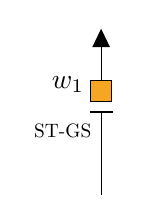
\begin{tikzpicture}[x=0.75pt,y=0.75pt,yscale=-1,xscale=1]
%uncomment if require: \path (0,300); %set diagram left start at 0, and has height of 300

%Shape: Rectangle [id:dp996418010681726] 
\draw  [fill={rgb, 255:red, 245; green, 166; blue, 35 }  ,fill opacity=1 ] (255,195) -- (265,195) -- (265,205) -- (255,205) -- cycle ;
%Straight Lines [id:da1931652613109811] 
\draw    (260,195) -- (260,172) ;
\draw [shift={(260,170)}, rotate = 450] [fill={rgb, 255:red, 0; green, 0; blue, 0 }  ][line width=0.75]  [draw opacity=0] (8.93,-4.29) -- (0,0) -- (8.93,4.29) -- cycle    ;

%Straight Lines [id:da14376405679335102] 
\draw    (260,250.2) -- (260,210) ;
\draw [shift={(260,210)}, rotate = 450] [color={rgb, 255:red, 0; green, 0; blue, 0 }  ][line width=0.75]    (0,5.59) -- (0,-5.59)   ;


% Text Node
\draw (244,197) node  [align=left] {$\displaystyle w_{1}$};
% Text Node
\draw (241.5,219) node [scale=0.7] [align=left] {ST-GS};
\end{tikzpicture}

\column{.90\textwidth}
The generation of a discrete token, $t$, from a vocabulary of $K$ tokens is achieved by sampling a categorical distribution 
\begin{equation*}
t \sim \operatorname{Cat}(p_1, \dots, p_K)\,; \,\sum_i p_i=1.
\end{equation*} \pause
Generating the probabilities $p_1, \dots, p_K$ directly from a neural network has potential numerical problems; it's much easier to generate un-normalised log-probabilities (logits), $x_1, \dots, x_K$. \pause
\\[0.5em]
The gumbel-softmax trick allows us to sample directly using the logits: 
\begin{equation*}
t = \underset{ i \in \{1,\cdots,K\} }{\operatorname{argmax}} x_i + z_i
\end{equation*}
where $z_1, \dots z_K$ are i.i.d Gumbel(0,1) variates  which can be computed from Uniform variates through $-\log(-\log(-\mathcal{U}(0,1)))$.
\end{columns}


\end{frame}

\begin{frame}
\frametitle{Differentiable Sampling: Straight-Through Gumbel Softmax}
Ok, but how does that help? $\operatorname{argmax}$ isn't differentiable! \pause
\\[0.5em]
...$\operatorname{softargmax}$ is:
\begin{equation*}
	\operatorname{softargmax}(\bm{y}) = \sum_i \frac{e^{\beta y_i}}{\sum_j e^{\beta y_j}} i
\end{equation*}

where $\beta$ is the inverse-temperature parameter. Higher values of $\beta$ give a more peaky distribution\footnote{in practice we'll either use an annealing schedule for the temperature, or just estimate a good value for a given $\bm{y}$ using an additional small network built into the model!}.
\end{frame}

\begin{frame}
\frametitle{Differentiable Sampling: Straight-Through Gumbel Softmax}
But... this clearly gives us a result that will be non-integer; we cannot round or clip because it would be non-differentiable. \pause
\\[0.5em]
The Straight-Through operator allows us to take the result of a true $\operatorname{argmax}$ that has the gradient of the $\operatorname{softargmax}$:
\begin{equation*}
	\operatorname{STargmax}(\bm{y}) = \operatorname{softargmax}(\bm{y}) + \operatorname{stopgradient}(\operatorname{argmax}(\bm{y}) - \operatorname{softargmax}(\bm{y})) 
\end{equation*}
where $\operatorname{stopgradient}$ is defined such that $\operatorname{stopgradient}(\bm{a}) = \bm{a}$ and $\nabla \operatorname{stopgradient}(\bm{a}) = 0$.
\pause
\begin{block}{Straight-Through Gumbel Softmax}
Combine the gumbel softmax trick with the $\operatorname{STargmax}$ to give you discrete samples, with a useable gradient\footnote{The ST operator is biased but low variance; in practice it works very well and is better than the high-variance unbiased estimates you could get through REINFORCE.}.
\end{block}

\end{frame}

\begin{frame}
\frametitle{How are we going to compute all the gradients needed for out optimiser?}
To solve optimisation problems using gradient methods we need to compute the gradients (derivatives) of the objective with respect to the parameters.
\\[0.5em]
In our model we're talking about the gradients of the hinge loss function, $\mathcal{L}$ with respect to the 6.2M parameters $\bm{\theta}$: $\nabla_{\bm{\theta}} \mathcal{L} = \frac{\partial \mathcal{L}}{\partial \bm{\theta}}$

\end{frame}

\begin{frame}
	\frametitle{Computing Derivatives}
There are three ways to compute derivatives:

\begin{columns}
	\column{.45\textwidth}
    \setbeamercovered{transparent}
    \begin{itemize}
    	\item<1,2> Symbolically differentiate the function with respect to its parameters
    	\begin{itemize}
    		\item by hand
    		\item using a CAS
    	\end{itemize}
    	\item<1,3> Make estimates using finite differences
    	\item<1,4> Use Automatic Differentiation
    \end{itemize}

    \column{.45\textwidth}
      \begin{block}{Problems}<2>
        Static - can't ``differentiate algorithms''; unwieldy with millions of variables
      \end{block}
      \begin{block}{Problems}<3>
        Numerical errors - will compound in deep nets
      \end{block}
  \end{columns}
\end{frame}

\begin{frame}
	\frametitle{What is Automatic Differentiation (AD)?}

	Automatic Differentiation is:
	\begin{itemize}
		\item a method to get exact derivatives efficiently, by storing information as you go forward that you can reuse as you go backwards.
		\begin{itemize}
			\item Takes code that computes a function and uses that to compute the derivative of that function.
		\item The goal isn't to obtain closed-form solutions, but to be able to write a program that efficiently computes the derivatives.
		\end{itemize}
	\end{itemize}
	\pause
	\begin{block}{Reverse-Mode Automatic Differentiation}
	Modern dynamic differentiable programming libraries are built around a technique called Reverse Mode Automatic Differentiation. 
	\\[0.5em]
	You write the forward pass; when you run the program, a `computation graph' can be built dynamically, and this graph contains the `adjoint variables' which can be used to compute gradients by applying the chain rule.
	\end{block}
\end{frame}

\begin{frame}
	\frametitle{Optimisation}

	\begin{columns}
	\setbeamercovered{transparent}
	\column{.45\textwidth}
	\begin{itemize}
		\item<1> We need to limit outselves to first-order methods.
		\item<2> Gradient Descent is conceptually simple.
		\item<3> Our loss landscape is wild.
	\end{itemize}
	\column{.45\textwidth}
	\begin{overprint}
	\setbeamercovered{invisible}
		\begin{block}{}<only@1>
			Computing the Hessian is not going to be feasible!
		\end{block}
		\begin{block}{}<only@2>
			Compute the gradient at the current point and take a step proportional to the gradient in the steepest direction.
		\end{block}
		\begin{block}{}<only@3>
			Utilise stochasticity to help explore (e.g. SGD).
			\\[0.5em]
			Utilise adaptive learning rates computed from the history of past moves ('momentum') to 'ride over bumps' - algorithms such as ADAM.
			\\[0.5em]
			Try to pick good starting points (e.g. He/Xavier(Glorot) initialisation).
			\\[0.5em]
			Use batch normalisation in the model to keep weights (and their gradients) in check.
		\end{block}
	\end{overprint}
	\end{columns}
\end{frame}

\begin{frame}
	\frametitle{Computation}
\begin{columns}

\column{.12\textwidth}

\centering
\includegraphics[width=0.8\columnwidth]{2080.jpg}\\
\includegraphics[width=0.8\columnwidth]{2080.jpg}\\
\includegraphics[width=0.8\columnwidth]{2080.jpg}\\
\includegraphics[width=0.8\columnwidth]{2080.jpg}\\

\column{.83\textwidth}

\begin{itemize}
	\setbeamercovered{transparent}
	\item<1> Our model is computationally extreme, yet we still would like to experiment with it in a reasonable amount of time.
	\item<1> GPUs which enabled the Deep Learning Revolution to start in 2012 are still just as relevant today.
	\item<2> Our model requires 4 RTX2080ti GPUs (each with 11G RAM) to run!
	\begin{itemize}
		\item The VGG16 backbone sits on one GPU
		\item The Sender and Reciever are each on a different GPU
		\item The loss computation takes place on the forth GPU
	\end{itemize}
	\item<2> For efficiency we use mini-batch SGD with ADAM to train
	\begin{itemize}
		\item mini-batch size of 128
		\item allows for 127 distractors and one target
		\item but we can utilise all 128 possible targets in a single iteration
	\end{itemize}
	\item<3> 74504 images in the training set; but this is made essentially infinite through data augmentation.
	\item<3> During training we can play and learn from 74496 games in about 7mins 30secs. It takes around 4 hours of play for convergence!
\end{itemize}	
\end{columns}
\end{frame}


\begin{frame}
\frametitle{Experiments}
In our NeuIPS EmeCom workshop paper\footfullcite{Mihai19} we explore \citeauthor{Havrylov2017}'s model under a number of different configurations.
\\[0.5em]
In all cases we shrunk the dataset to 32x32 images from the CIFAR-10 dataset, reduced the allowed vocabulary size to 100 tokens, and setting the maximum sentence length to 5.
\begin{itemize}
	\item This makes the model much more manageable - you can \emph{just} fit the whole thing on open GPU with 127 distractors + 1 target.\\[1em]
\end{itemize}
% \\[0.5em]
\pause
Key metrics are:  \\
\centering
\begin{tabular}{ll}
\hline
Comm. success rate & proportion of fully successfully games\\
Top-5 comm. success rate & proportion of almost successful games\\
\#target class in top-5 & \#images in the top five with target label\\
Target class avg. rank & average rank of images with the target label\\ \hline
\end{tabular}
\end{frame}

\begin{frame}
\frametitle{Experiments \& Findings 1: feature extraction}
We firstly explored the importance of the VGG16 feature extraction network, and explored the effect of \begin{itemize}
		\item learning it as part of the model;
		\item keeping it fixed with random weights; and
		\item keeping it fixed with pretrained weights from ImageNet (essentially `importing' external semantic knowledge into the network).  \\[1em]
\end{itemize}
\pause
\centering
\begin{tabular}{llllll}
\hline
 Feature extractor & Comm. & Top-5 & \#target-class  & Target-class \\
   & rate & comm. rate & in top-5 & avg. rank \\ \hline
 Pretrained \& fixed & 0.88 ($\pm$0.31) &0.99 &1.84 &46.58\\

 Random \& frozen &0.95 ($\pm$0.19) &1 &1.66 &52.13\\

Learned end-end &0.89 ($\pm$0.3) &1 &1.53 &54.01\\ \hline
\end{tabular}

\begin{block}{}
Visual semantics are much stronger in the pretrained model, but they don't make for the best game-play. A fully learned model doesn't learn any notion of semantics.
\end{block}

\end{frame}

\begin{frame}
\frametitle{Experiments \& Findings 2: augmentation}
We then explored the effect of using augmentations to make the game harder.\\[1em]
\pause
\centering
\begin{tabular}{llllll}
\hline
 Feature extractor & Comm. & Top-5 & \#target-class  & Target-class \\
   & rate & comm. rate & in top-5 & avg. rank \\
\hline
\multicolumn{5}{l}{\textbf{Sender images augmented with Gaussian noise:}}\\
  Pretrained \& fixed & 0.92 ($\pm$0.26) & 0.99 & 1.85 & 46.12\\

  Random \& frozen & 0.96 ($\pm$0.19) & 1 & 1.6 & 54.01\\

  Learned end-end & 0.94 ($\pm$0.23) & 1 & 1.5 & 57.11\\
\hline
\multicolumn{5}{l}{\textbf{Sender images augmented with random rotations:}}\\
  Pretrained \& fixed & 0.83 ($\pm$0.37) & 0.99 &2.07 &41.89\\

  Random \& frozen & 0.87 ($\pm$0.33) & 0.99 &1.7 &51.89\\

  Learned end-end & 0.92 ($\pm$0.25) & 1 & 1.6 &55.96\\
\hline
\end{tabular}

\begin{block}{}
Adding noise makes the communication rate increase; adding rotations makes the semantics increase (but decreases communication success rate).
\end{block}

\end{frame}

\begin{frame}
\frametitle{Experiments \& Findings 3: multiple tasks}
Finally we extended the game to include a secondary task (guessing the rotation of the sender's input) in order to assess whether having agents perform more diverse tasks might lead to stronger visual semantics emerging.
\begin{figure}
    \centering
    \begin{tabular}{c@{\hskip 1in}c}
    \resizebox{0.3\textwidth}{!}{\input{model-rot.tikz}\unskip} &
    \resizebox{0.3\textwidth}{!}{

\tikzset{every picture/.style={line width=0.75pt}} %set default line width to 0.75pt        

\begin{tikzpicture}[x=0.75pt,y=0.75pt,yscale=-1,xscale=1]
%uncomment if require: \path (0,463); %set diagram left start at 0, and has height of 463

%Shape: Rectangle [id:dp2990102139159513] 
\draw  [fill={rgb, 255:red, 126; green, 211; blue, 33 }  ,fill opacity=1 ] (235,155.2) -- (245,155.2) -- (245,195.2) -- (235,195.2) -- cycle ;
%Shape: Rectangle [id:dp8784771675534407] 
\draw  [fill={rgb, 255:red, 126; green, 211; blue, 33 }  ,fill opacity=1 ] (285,155.2) -- (295,155.2) -- (295,195.2) -- (285,195.2) -- cycle ;
%Shape: Rectangle [id:dp11751835806588318] 
\draw  [fill={rgb, 255:red, 126; green, 211; blue, 33 }  ,fill opacity=1 ] (335,155.2) -- (345,155.2) -- (345,195.2) -- (335,195.2) -- cycle ;
%Shape: Rectangle [id:dp5110140830291819] 
\draw  [fill={rgb, 255:red, 126; green, 211; blue, 33 }  ,fill opacity=1 ] (385,155.2) -- (395,155.2) -- (395,195.2) -- (385,195.2) -- cycle ;
%Shape: Rectangle [id:dp8336305242746987] 
\draw  [fill={rgb, 255:red, 126; green, 211; blue, 33 }  ,fill opacity=1 ] (435,155.2) -- (445,155.2) -- (445,195.2) -- (435,195.2) -- cycle ;
%Shape: Rectangle [id:dp4962642966607703] 
\draw  [fill={rgb, 255:red, 74; green, 144; blue, 226 }  ,fill opacity=1 ] (235,305.2) -- (245,305.2) -- (245,345.2) -- (235,345.2) -- cycle ;
%Shape: Rectangle [id:dp351100809926032] 
\draw  [fill={rgb, 255:red, 74; green, 144; blue, 226 }  ,fill opacity=1 ] (285,305.2) -- (295,305.2) -- (295,345.2) -- (285,345.2) -- cycle ;
%Shape: Rectangle [id:dp02453276479923272] 
\draw  [fill={rgb, 255:red, 74; green, 144; blue, 226 }  ,fill opacity=1 ] (335,305.2) -- (345,305.2) -- (345,345.2) -- (335,345.2) -- cycle ;
%Shape: Rectangle [id:dp18135675144546226] 
\draw  [fill={rgb, 255:red, 74; green, 144; blue, 226 }  ,fill opacity=1 ] (385,305.2) -- (395,305.2) -- (395,345.2) -- (385,345.2) -- cycle ;
%Shape: Rectangle [id:dp9085096667905425] 
\draw  [fill={rgb, 255:red, 74; green, 144; blue, 226 }  ,fill opacity=1 ] (435,305.2) -- (445,305.2) -- (445,345.2) -- (435,345.2) -- cycle ;
%Shape: Rectangle [id:dp46627372731091776] 
\draw  [fill={rgb, 255:red, 74; green, 144; blue, 226 }  ,fill opacity=1 ] (185,305.2) -- (195,305.2) -- (195,345.2) -- (185,345.2) -- cycle ;
%Shape: Rectangle [id:dp6011323267929616] 
\draw  [fill={rgb, 255:red, 208; green, 2; blue, 27 }  ,fill opacity=1 ] (235,215) -- (245,215) -- (245,225) -- (235,225) -- cycle ;
%Shape: Rectangle [id:dp3631501371372986] 
\draw  [fill={rgb, 255:red, 208; green, 2; blue, 27 }  ,fill opacity=1 ] (335,215) -- (345,215) -- (345,225) -- (335,225) -- cycle ;
%Shape: Rectangle [id:dp37347060104166074] 
\draw  [fill={rgb, 255:red, 208; green, 2; blue, 27 }  ,fill opacity=1 ] (285,215) -- (295,215) -- (295,225) -- (285,225) -- cycle ;
%Shape: Rectangle [id:dp15668986272908303] 
\draw  [fill={rgb, 255:red, 208; green, 2; blue, 27 }  ,fill opacity=1 ] (385,215.2) -- (395,215.2) -- (395,225.2) -- (385,225.2) -- cycle ;
%Shape: Rectangle [id:dp9546093964256938] 
\draw  [fill={rgb, 255:red, 208; green, 2; blue, 27 }  ,fill opacity=1 ] (435,215) -- (445,215) -- (445,225) -- (435,225) -- cycle ;
%Shape: Rectangle [id:dp6440027515701122] 
\draw  [fill={rgb, 255:red, 245; green, 166; blue, 35 }  ,fill opacity=1 ] (235,250) -- (245,250) -- (245,260) -- (235,260) -- cycle ;
%Shape: Rectangle [id:dp9765020857760711] 
\draw  [fill={rgb, 255:red, 245; green, 166; blue, 35 }  ,fill opacity=1 ] (335,250) -- (345,250) -- (345,260) -- (335,260) -- cycle ;
%Shape: Rectangle [id:dp6847537038373258] 
\draw  [fill={rgb, 255:red, 245; green, 166; blue, 35 }  ,fill opacity=1 ] (285,250) -- (295,250) -- (295,260) -- (285,260) -- cycle ;
%Shape: Rectangle [id:dp6254432051412727] 
\draw  [fill={rgb, 255:red, 245; green, 166; blue, 35 }  ,fill opacity=1 ] (385,250) -- (395,250) -- (395,260) -- (385,260) -- cycle ;
%Shape: Rectangle [id:dp28896388671746975] 
\draw  [fill={rgb, 255:red, 245; green, 166; blue, 35 }  ,fill opacity=1 ] (435,250) -- (445,250) -- (445,260) -- (435,260) -- cycle ;
%Shape: Rectangle [id:dp2901739846228756] 
\draw  [fill={rgb, 255:red, 189; green, 16; blue, 224 }  ,fill opacity=1 ] (235,365.2) -- (245,365.2) -- (245,375.2) -- (235,375.2) -- cycle ;
%Shape: Rectangle [id:dp8060114453218804] 
\draw  [fill={rgb, 255:red, 189; green, 16; blue, 224 }  ,fill opacity=1 ] (335,365.2) -- (345,365.2) -- (345,375.2) -- (335,375.2) -- cycle ;
%Shape: Rectangle [id:dp31679742893495677] 
\draw  [fill={rgb, 255:red, 189; green, 16; blue, 224 }  ,fill opacity=1 ] (285,365.2) -- (295,365.2) -- (295,375.2) -- (285,375.2) -- cycle ;
%Shape: Rectangle [id:dp6003994298629624] 
\draw  [fill={rgb, 255:red, 189; green, 16; blue, 224 }  ,fill opacity=1 ] (385,365.2) -- (395,365.2) -- (395,375.2) -- (385,375.2) -- cycle ;
%Shape: Rectangle [id:dp019292076660878732] 
\draw  [fill={rgb, 255:red, 189; green, 16; blue, 224 }  ,fill opacity=1 ] (435,365.2) -- (445,365.2) -- (445,375.2) -- (435,375.2) -- cycle ;
%Straight Lines [id:da8460185543636454] 
\draw    (195,325.2) -- (233,325.2) ;
\draw [shift={(235,325.2)}, rotate = 180] [fill={rgb, 255:red, 0; green, 0; blue, 0 }  ][line width=0.75]  [draw opacity=0] (8.93,-4.29) -- (0,0) -- (8.93,4.29) -- cycle    ;

%Straight Lines [id:da8340795876607023] 
\draw    (245,325.2) -- (283,325.2) ;
\draw [shift={(285,325.2)}, rotate = 180] [fill={rgb, 255:red, 0; green, 0; blue, 0 }  ][line width=0.75]  [draw opacity=0] (8.93,-4.29) -- (0,0) -- (8.93,4.29) -- cycle    ;

%Straight Lines [id:da01318748080001153] 
\draw    (295,325.2) -- (333,325.2) ;
\draw [shift={(335,325.2)}, rotate = 180] [fill={rgb, 255:red, 0; green, 0; blue, 0 }  ][line width=0.75]  [draw opacity=0] (8.93,-4.29) -- (0,0) -- (8.93,4.29) -- cycle    ;

%Straight Lines [id:da5338983303988957] 
\draw    (345,325.2) -- (383,325.2) ;
\draw [shift={(385,325.2)}, rotate = 180] [fill={rgb, 255:red, 0; green, 0; blue, 0 }  ][line width=0.75]  [draw opacity=0] (8.93,-4.29) -- (0,0) -- (8.93,4.29) -- cycle    ;

%Straight Lines [id:da9598890254070799] 
\draw    (395,325.2) -- (433,325.2) ;
\draw [shift={(435,325.2)}, rotate = 180] [fill={rgb, 255:red, 0; green, 0; blue, 0 }  ][line width=0.75]  [draw opacity=0] (8.93,-4.29) -- (0,0) -- (8.93,4.29) -- cycle    ;

%Straight Lines [id:da8053105047556711] 
\draw    (240,365.2) -- (240,347.2) ;
\draw [shift={(240,345.2)}, rotate = 450] [fill={rgb, 255:red, 0; green, 0; blue, 0 }  ][line width=0.75]  [draw opacity=0] (8.93,-4.29) -- (0,0) -- (8.93,4.29) -- cycle    ;

%Straight Lines [id:da6073538607686498] 
\draw    (290,365.2) -- (290,347.2) ;
\draw [shift={(290,345.2)}, rotate = 450] [fill={rgb, 255:red, 0; green, 0; blue, 0 }  ][line width=0.75]  [draw opacity=0] (8.93,-4.29) -- (0,0) -- (8.93,4.29) -- cycle    ;

%Straight Lines [id:da7269219133762375] 
\draw    (340,365.2) -- (340,347.2) ;
\draw [shift={(340,345.2)}, rotate = 450] [fill={rgb, 255:red, 0; green, 0; blue, 0 }  ][line width=0.75]  [draw opacity=0] (8.93,-4.29) -- (0,0) -- (8.93,4.29) -- cycle    ;

%Straight Lines [id:da3739045253711666] 
\draw    (390,365.2) -- (390,347.2) ;
\draw [shift={(390,345.2)}, rotate = 450] [fill={rgb, 255:red, 0; green, 0; blue, 0 }  ][line width=0.75]  [draw opacity=0] (8.93,-4.29) -- (0,0) -- (8.93,4.29) -- cycle    ;

%Straight Lines [id:da6326771747088481] 
\draw    (440,365.2) -- (440,347.2) ;
\draw [shift={(440,345.2)}, rotate = 450] [fill={rgb, 255:red, 0; green, 0; blue, 0 }  ][line width=0.75]  [draw opacity=0] (8.93,-4.29) -- (0,0) -- (8.93,4.29) -- cycle    ;

%Straight Lines [id:da7550754427915821] 
\draw    (240,250) -- (240,227) ;
\draw [shift={(240,225)}, rotate = 450] [fill={rgb, 255:red, 0; green, 0; blue, 0 }  ][line width=0.75]  [draw opacity=0] (8.93,-4.29) -- (0,0) -- (8.93,4.29) -- cycle    ;

%Straight Lines [id:da810548383269696] 
\draw    (240,215.2) -- (240,197.2) ;
\draw [shift={(240,195.2)}, rotate = 450] [fill={rgb, 255:red, 0; green, 0; blue, 0 }  ][line width=0.75]  [draw opacity=0] (8.93,-4.29) -- (0,0) -- (8.93,4.29) -- cycle    ;

%Straight Lines [id:da5748135260636472] 
\draw    (290,250) -- (290,227.2) ;
\draw [shift={(290,225.2)}, rotate = 450] [fill={rgb, 255:red, 0; green, 0; blue, 0 }  ][line width=0.75]  [draw opacity=0] (8.93,-4.29) -- (0,0) -- (8.93,4.29) -- cycle    ;

%Straight Lines [id:da4933542699121286] 
\draw    (290,215.2) -- (290,197.2) ;
\draw [shift={(290,195.2)}, rotate = 450] [fill={rgb, 255:red, 0; green, 0; blue, 0 }  ][line width=0.75]  [draw opacity=0] (8.93,-4.29) -- (0,0) -- (8.93,4.29) -- cycle    ;

%Straight Lines [id:da574033058980986] 
\draw    (340,250) -- (340,227.2) ;
\draw [shift={(340,225.2)}, rotate = 450] [fill={rgb, 255:red, 0; green, 0; blue, 0 }  ][line width=0.75]  [draw opacity=0] (8.93,-4.29) -- (0,0) -- (8.93,4.29) -- cycle    ;

%Straight Lines [id:da40655794814262236] 
\draw    (340,215.2) -- (340,197.2) ;
\draw [shift={(340,195.2)}, rotate = 450] [fill={rgb, 255:red, 0; green, 0; blue, 0 }  ][line width=0.75]  [draw opacity=0] (8.93,-4.29) -- (0,0) -- (8.93,4.29) -- cycle    ;

%Straight Lines [id:da3550375711507877] 
\draw    (390,250) -- (390,227.2) ;
\draw [shift={(390,225.2)}, rotate = 450] [fill={rgb, 255:red, 0; green, 0; blue, 0 }  ][line width=0.75]  [draw opacity=0] (8.93,-4.29) -- (0,0) -- (8.93,4.29) -- cycle    ;

%Straight Lines [id:da40454484083266984] 
\draw    (390,215) -- (390,197) ;
\draw [shift={(390,195)}, rotate = 450] [fill={rgb, 255:red, 0; green, 0; blue, 0 }  ][line width=0.75]  [draw opacity=0] (8.93,-4.29) -- (0,0) -- (8.93,4.29) -- cycle    ;

%Straight Lines [id:da15757045692999683] 
\draw    (440,250) -- (440,227.2) ;
\draw [shift={(440,225.2)}, rotate = 450] [fill={rgb, 255:red, 0; green, 0; blue, 0 }  ][line width=0.75]  [draw opacity=0] (8.93,-4.29) -- (0,0) -- (8.93,4.29) -- cycle    ;

%Straight Lines [id:da440695876559432] 
\draw    (440,215.2) -- (440,197.2) ;
\draw [shift={(440,195.2)}, rotate = 450] [fill={rgb, 255:red, 0; green, 0; blue, 0 }  ][line width=0.75]  [draw opacity=0] (8.93,-4.29) -- (0,0) -- (8.93,4.29) -- cycle    ;

%Straight Lines [id:da5803361900921704] 
\draw    (245,175.2) -- (283,175.2) ;
\draw [shift={(285,175.2)}, rotate = 180] [fill={rgb, 255:red, 0; green, 0; blue, 0 }  ][line width=0.75]  [draw opacity=0] (8.93,-4.29) -- (0,0) -- (8.93,4.29) -- cycle    ;

%Straight Lines [id:da4030513421969921] 
\draw    (295,175.2) -- (333,175.2) ;
\draw [shift={(335,175.2)}, rotate = 180] [fill={rgb, 255:red, 0; green, 0; blue, 0 }  ][line width=0.75]  [draw opacity=0] (8.93,-4.29) -- (0,0) -- (8.93,4.29) -- cycle    ;

%Straight Lines [id:da42554182247229266] 
\draw    (345,175.2) -- (383,175.2) ;
\draw [shift={(385,175.2)}, rotate = 180] [fill={rgb, 255:red, 0; green, 0; blue, 0 }  ][line width=0.75]  [draw opacity=0] (8.93,-4.29) -- (0,0) -- (8.93,4.29) -- cycle    ;

%Straight Lines [id:da6818428411432212] 
\draw    (395,175.2) -- (433,175.2) ;
\draw [shift={(435,175.2)}, rotate = 180] [fill={rgb, 255:red, 0; green, 0; blue, 0 }  ][line width=0.75]  [draw opacity=0] (8.93,-4.29) -- (0,0) -- (8.93,4.29) -- cycle    ;

%Straight Lines [id:da7554494867186758] 
\draw    (240,305.2) -- (240,265) ;
\draw [shift={(240,265)}, rotate = 450] [color={rgb, 255:red, 0; green, 0; blue, 0 }  ][line width=0.75]    (0,5.59) -- (0,-5.59)   ;

%Straight Lines [id:da8051297860745438] 
\draw    (290,305.2) -- (290,265) ;
\draw [shift={(290,265)}, rotate = 450] [color={rgb, 255:red, 0; green, 0; blue, 0 }  ][line width=0.75]    (0,5.59) -- (0,-5.59)   ;

%Straight Lines [id:da9067183857475836] 
\draw    (340,305.2) -- (340,265) ;
\draw [shift={(340,265)}, rotate = 450] [color={rgb, 255:red, 0; green, 0; blue, 0 }  ][line width=0.75]    (0,5.59) -- (0,-5.59)   ;

%Straight Lines [id:da14177597111404827] 
\draw    (390,305.2) -- (390,265) ;
\draw [shift={(390,265)}, rotate = 450] [color={rgb, 255:red, 0; green, 0; blue, 0 }  ][line width=0.75]    (0,5.59) -- (0,-5.59)   ;

%Straight Lines [id:da8699775338311366] 
\draw    (440,305.2) -- (440,265) ;
\draw [shift={(440,265)}, rotate = 450] [color={rgb, 255:red, 0; green, 0; blue, 0 }  ][line width=0.75]    (0,5.59) -- (0,-5.59)   ;

%Curve Lines [id:da027202656987267093] 
\draw  [dash pattern={on 0.84pt off 2.51pt}]  (245,255) .. controls (250.01,255.25) and (260.41,254.45) .. (260,320) .. controls (259.6,384.56) and (289.74,416.24) .. (290.01,377.04) ;
\draw [shift={(290,375.2)}, rotate = 449.09] [fill={rgb, 255:red, 0; green, 0; blue, 0 }  ][line width=0.75]  [draw opacity=0] (8.93,-4.29) -- (0,0) -- (8.93,4.29) -- cycle    ;

%Flowchart: Manual Operation [id:dp9480879498998894] 
\draw  [fill={rgb, 255:red, 248; green, 231; blue, 28 }  ,fill opacity=1 ] (110.06,340.81) -- (80,350) -- (80.3,300) -- (110.25,309.56) -- cycle ;
%Shape: Rectangle [id:dp55444069879049] 
\draw  [fill={rgb, 255:red, 139; green, 87; blue, 42 }  ,fill opacity=1 ] (135,345.06) -- (125,345) -- (125.24,305) -- (135.24,305.06) -- cycle ;
%Straight Lines [id:da023195017403435325] 
\draw    (160,325) -- (183,325) ;
\draw [shift={(185,325)}, rotate = 180] [fill={rgb, 255:red, 0; green, 0; blue, 0 }  ][line width=0.75]  [draw opacity=0] (8.93,-4.29) -- (0,0) -- (8.93,4.29) -- cycle    ;

%Straight Lines [id:da3640080622227335] 
\draw    (110,324.8) -- (123,324.97) ;
\draw [shift={(125,325)}, rotate = 180.76] [fill={rgb, 255:red, 0; green, 0; blue, 0 }  ][line width=0.75]  [draw opacity=0] (8.93,-4.29) -- (0,0) -- (8.93,4.29) -- cycle    ;

%Straight Lines [id:da9694174603040991] 
\draw    (55,324.8) -- (78,324.8) ;
\draw [shift={(80,324.8)}, rotate = 180] [fill={rgb, 255:red, 0; green, 0; blue, 0 }  ][line width=0.75]  [draw opacity=0] (8.93,-4.29) -- (0,0) -- (8.93,4.29) -- cycle    ;

%Shape: Rectangle [id:dp37158497488699105] 
\draw  [color={rgb, 255:red, 155; green, 155; blue, 155 }  ,draw opacity=1 ] (0,240) -- (450,240) -- (450,410) -- (0,410) -- cycle ;
%Shape: Rectangle [id:dp8414177271165663] 
\draw  [fill={rgb, 255:red, 80; green, 227; blue, 194 }  ,fill opacity=1 ] (159.76,345.06) -- (149.76,345) -- (150,305) -- (160,305.06) -- cycle ;
%Straight Lines [id:da6455282380830417] 
\draw    (135.15,325.37) -- (148,325.05) ;
\draw [shift={(150,325)}, rotate = 538.5799999999999] [fill={rgb, 255:red, 0; green, 0; blue, 0 }  ][line width=0.75]  [draw opacity=0] (8.93,-4.29) -- (0,0) -- (8.93,4.29) -- cycle    ;

%Shape: Rectangle [id:dp4069916382636678] 
\draw  [color={rgb, 255:red, 155; green, 155; blue, 155 }  ,draw opacity=1 ] (175,85) -- (660,85) -- (660,280) -- (175,280) -- cycle ;
%Image [id:dp7681395321021224] 
\draw (35.15,324.85) node [rotate=-270] {\includegraphics[width=37.27pt,height=37.73pt]{automobile4.png}};
%Straight Lines [id:da14896127984865282] 
\draw    (240,395) -- (240,377) ;
\draw [shift={(240,375)}, rotate = 450] [fill={rgb, 255:red, 0; green, 0; blue, 0 }  ][line width=0.75]  [draw opacity=0] (8.93,-4.29) -- (0,0) -- (8.93,4.29) -- cycle    ;

%Flowchart: Manual Operation [id:dp44022383265143505] 
\draw  [fill={rgb, 255:red, 248; green, 193; blue, 28 }  ,fill opacity=1 ] (140,281.5) -- (125,289) -- (125,249) -- (140,256.5) -- cycle ;
%Curve Lines [id:da5124282022015486] 
\draw    (110,324.8) .. controls (135.12,297.42) and (89.89,270.81) .. (123.41,269.06) ;
\draw [shift={(125,269)}, rotate = 538.4300000000001] [fill={rgb, 255:red, 0; green, 0; blue, 0 }  ][line width=0.75]  [draw opacity=0] (8.93,-4.29) -- (0,0) -- (8.93,4.29) -- cycle    ;

%Straight Lines [id:da979793122680816] 
\draw    (140,268.39) -- (158,268.39) ;
\draw [shift={(160,268.39)}, rotate = 180] [fill={rgb, 255:red, 0; green, 0; blue, 0 }  ][line width=0.75]  [draw opacity=0] (8.93,-4.29) -- (0,0) -- (8.93,4.29) -- cycle    ;

%Shape: Circle [id:dp4109130775703994] 
\draw   (170,268.39) .. controls (170,265.63) and (167.76,263.39) .. (165,263.39) .. controls (162.24,263.39) and (160,265.63) .. (160,268.39) .. controls (160,271.15) and (162.24,273.39) .. (165,273.39) .. controls (167.76,273.39) and (170,271.15) .. (170,268.39) -- cycle ;
%Curve Lines [id:da9459923233179771] 
\draw  [dash pattern={on 4.5pt off 4.5pt}]  (75,100) .. controls (75,88) and (76.5,172) .. (75,230) .. controls (73.52,287.13) and (37.6,261.79) .. (35.09,298.29) ;
\draw [shift={(35,300)}, rotate = 272.2] [fill={rgb, 255:red, 0; green, 0; blue, 0 }  ][line width=0.75]  [draw opacity=0] (8.93,-4.29) -- (0,0) -- (8.93,4.29) -- cycle    ;

%Curve Lines [id:da3371187008420946] 
\draw  [dash pattern={on 4.5pt off 4.5pt}]  (75,100) .. controls (75,88.12) and (163.7,202.67) .. (164.99,261.62) ;
\draw [shift={(165,263.39)}, rotate = 270.49] [fill={rgb, 255:red, 0; green, 0; blue, 0 }  ][line width=0.75]  [draw opacity=0] (8.93,-4.29) -- (0,0) -- (8.93,4.29) -- cycle    ;

%Curve Lines [id:da534752150197891] 
\draw  [dash pattern={on 0.84pt off 2.51pt}]  (295,255) .. controls (300.01,255.25) and (310.41,254.45) .. (310,320) .. controls (309.6,384.56) and (339.74,416.24) .. (340.01,377.04) ;
\draw [shift={(340,375.2)}, rotate = 449.09] [fill={rgb, 255:red, 0; green, 0; blue, 0 }  ][line width=0.75]  [draw opacity=0] (8.93,-4.29) -- (0,0) -- (8.93,4.29) -- cycle    ;

%Curve Lines [id:da20471705420640562] 
\draw  [dash pattern={on 0.84pt off 2.51pt}]  (345,255) .. controls (350.01,255.25) and (360.41,254.45) .. (360,320) .. controls (359.6,384.56) and (389.74,416.24) .. (390.01,377.04) ;
\draw [shift={(390,375.2)}, rotate = 449.09] [fill={rgb, 255:red, 0; green, 0; blue, 0 }  ][line width=0.75]  [draw opacity=0] (8.93,-4.29) -- (0,0) -- (8.93,4.29) -- cycle    ;

%Curve Lines [id:da239328274527008] 
\draw  [dash pattern={on 0.84pt off 2.51pt}]  (395,255) .. controls (400.01,255.25) and (410.41,254.45) .. (410,320) .. controls (409.6,384.56) and (439.74,416.24) .. (440.01,377.04) ;
\draw [shift={(440,375.2)}, rotate = 449.09] [fill={rgb, 255:red, 0; green, 0; blue, 0 }  ][line width=0.75]  [draw opacity=0] (8.93,-4.29) -- (0,0) -- (8.93,4.29) -- cycle    ;

%Flowchart: Manual Operation [id:dp5102273317705665] 
\draw  [fill={rgb, 255:red, 248; green, 231; blue, 28 }  ,fill opacity=1 ] (560,219.07) -- (590,209.7) -- (590,259.7) -- (560,250.32) -- cycle ;
%Flowchart: Manual Operation [id:dp5169291677953056] 
\draw  [fill={rgb, 255:red, 248; green, 231; blue, 28 }  ,fill opacity=1 ] (560,159.07) -- (590,149.7) -- (590,199.7) -- (560,190.32) -- cycle ;
%Flowchart: Manual Operation [id:dp8211654659347366] 
\draw  [fill={rgb, 255:red, 248; green, 231; blue, 28 }  ,fill opacity=1 ] (560,99.07) -- (590,89.7) -- (590,139.7) -- (560,130.32) -- cycle ;
%Straight Lines [id:da3846010305229277] 
\draw    (605,114.7) -- (592,114.7) ;
\draw [shift={(590,114.7)}, rotate = 360] [fill={rgb, 255:red, 0; green, 0; blue, 0 }  ][line width=0.75]  [draw opacity=0] (8.93,-4.29) -- (0,0) -- (8.93,4.29) -- cycle    ;

%Straight Lines [id:da470672840529025] 
\draw    (605,174.7) -- (592,174.7) ;
\draw [shift={(590,174.7)}, rotate = 360] [fill={rgb, 255:red, 0; green, 0; blue, 0 }  ][line width=0.75]  [draw opacity=0] (8.93,-4.29) -- (0,0) -- (8.93,4.29) -- cycle    ;

%Straight Lines [id:da7653958928086578] 
\draw    (605,234.7) -- (592,234.7) ;
\draw [shift={(590,234.7)}, rotate = 360] [fill={rgb, 255:red, 0; green, 0; blue, 0 }  ][line width=0.75]  [draw opacity=0] (8.93,-4.29) -- (0,0) -- (8.93,4.29) -- cycle    ;

%Straight Lines [id:da24697789431854034] 
\draw    (560,234.7) -- (547,234.7) ;
\draw [shift={(545,234.7)}, rotate = 360] [fill={rgb, 255:red, 0; green, 0; blue, 0 }  ][line width=0.75]  [draw opacity=0] (8.93,-4.29) -- (0,0) -- (8.93,4.29) -- cycle    ;

%Straight Lines [id:da7486447676597899] 
\draw    (560,174.7) -- (547,174.7) ;
\draw [shift={(545,174.7)}, rotate = 360] [fill={rgb, 255:red, 0; green, 0; blue, 0 }  ][line width=0.75]  [draw opacity=0] (8.93,-4.29) -- (0,0) -- (8.93,4.29) -- cycle    ;

%Straight Lines [id:da7472608495765627] 
\draw    (560,114.7) -- (547,114.7) ;
\draw [shift={(545,114.7)}, rotate = 360] [fill={rgb, 255:red, 0; green, 0; blue, 0 }  ][line width=0.75]  [draw opacity=0] (8.93,-4.29) -- (0,0) -- (8.93,4.29) -- cycle    ;

%Shape: Circle [id:dp604734065579139] 
\draw   (545,114.7) .. controls (545,111.93) and (542.76,109.7) .. (540,109.7) .. controls (537.24,109.7) and (535,111.93) .. (535,114.7) .. controls (535,117.46) and (537.24,119.7) .. (540,119.7) .. controls (542.76,119.7) and (545,117.46) .. (545,114.7) -- cycle ;
%Shape: Circle [id:dp1913469612555806] 
\draw   (545,174.7) .. controls (545,171.93) and (542.76,169.7) .. (540,169.7) .. controls (537.24,169.7) and (535,171.93) .. (535,174.7) .. controls (535,177.46) and (537.24,179.7) .. (540,179.7) .. controls (542.76,179.7) and (545,177.46) .. (545,174.7) -- cycle ;
%Shape: Circle [id:dp6888026181324974] 
\draw   (545,234.7) .. controls (545,231.93) and (542.76,229.7) .. (540,229.7) .. controls (537.24,229.7) and (535,231.93) .. (535,234.7) .. controls (535,237.46) and (537.24,239.7) .. (540,239.7) .. controls (542.76,239.7) and (545,237.46) .. (545,234.7) -- cycle ;
%Curve Lines [id:da4657611124859501] 
\draw    (499.88,174.73) .. controls (528.44,174.73) and (499.88,117.13) .. (533.42,114.76) ;
\draw [shift={(535,114.7)}, rotate = 538.94] [fill={rgb, 255:red, 0; green, 0; blue, 0 }  ][line width=0.75]  [draw opacity=0] (8.93,-4.29) -- (0,0) -- (8.93,4.29) -- cycle    ;

%Curve Lines [id:da43245208412763236] 
\draw    (499.88,174.73) .. controls (528.44,174.73) and (499.88,233.56) .. (533.42,234.68) ;
\draw [shift={(535,234.7)}, rotate = 538.94] [fill={rgb, 255:red, 0; green, 0; blue, 0 }  ][line width=0.75]  [draw opacity=0] (8.93,-4.29) -- (0,0) -- (8.93,4.29) -- cycle    ;

%Straight Lines [id:da60878364805108] 
\draw    (499.88,174.73) -- (533,174.7) ;
\draw [shift={(535,174.7)}, rotate = 539.95] [fill={rgb, 255:red, 0; green, 0; blue, 0 }  ][line width=0.75]  [draw opacity=0] (8.93,-4.29) -- (0,0) -- (8.93,4.29) -- cycle    ;

%Straight Lines [id:da15523941632201144] 
\draw    (445,174.7) -- (463,174.7) ;
\draw [shift={(465,174.7)}, rotate = 180] [fill={rgb, 255:red, 0; green, 0; blue, 0 }  ][line width=0.75]  [draw opacity=0] (8.93,-4.29) -- (0,0) -- (8.93,4.29) -- cycle    ;

%Image [id:dp17468911895914307] 
\draw (629.85,234.85) node  {\includegraphics[width=37.27pt,height=37.73pt]{automobile4.png}};
%Image [id:dp7963562409170879] 
\draw (630,114.7) node  {\includegraphics[width=37.5pt,height=37.5pt]{horse5.png}};
%Image [id:dp1715536820396606] 
\draw (630,174.7) node  {\includegraphics[width=37.5pt,height=37.5pt]{ship1.png}};
%Shape: Rectangle [id:dp7854500427526406] 
\draw  [fill={rgb, 255:red, 184; green, 233; blue, 134 }  ,fill opacity=1 ] (474.76,194.76) -- (464.76,194.69) -- (465,154.7) -- (475,154.76) -- cycle ;
%Straight Lines [id:da4610299418428241] 
\draw    (475,174.7) -- (493,174.7) ;
\draw [shift={(495,174.7)}, rotate = 180] [fill={rgb, 255:red, 0; green, 0; blue, 0 }  ][line width=0.75]  [draw opacity=0] (8.93,-4.29) -- (0,0) -- (8.93,4.29) -- cycle    ;

%Shape: Rectangle [id:dp0526782408589167] 
\draw  [fill={rgb, 255:red, 82; green, 2; blue, 208 }  ,fill opacity=1 ] (494.88,154.73) -- (504.88,154.73) -- (504.88,194.73) -- (494.88,194.73) -- cycle ;

% Text Node
\draw (224,152.7) node  [align=left] {$\displaystyle h^{r}_{1}$};
% Text Node
\draw (274,152.5) node  [align=left] {$\displaystyle h^{r}_{2}$};
% Text Node
\draw (324,152.7) node  [align=left] {$\displaystyle h^{r}_{3}$};
% Text Node
\draw (374,152.7) node  [align=left] {$\displaystyle h^{r}_{4}$};
% Text Node
\draw (424,152.7) node  [align=left] {$\displaystyle h^{r}_{5}$};
% Text Node
\draw (224,302.5) node  [align=left] {$\displaystyle h^{s}_{1}$};
% Text Node
\draw (274,302.5) node  [align=left] {$\displaystyle h^{s}_{2}$};
% Text Node
\draw (322,302.5) node  [align=left] {$\displaystyle h^{s}_{3}$};
% Text Node
\draw (372,302.5) node  [align=left] {$\displaystyle h^{s}_{4}$};
% Text Node
\draw (422,302.5) node  [align=left] {$\displaystyle h^{s}_{5}$};
% Text Node
\draw (176,302.7) node  [align=left] {$\displaystyle h^{s}_{0}$};
% Text Node
\draw (224,252) node  [align=left] {$\displaystyle w_{1}$};
% Text Node
\draw (274,252) node  [align=left] {$\displaystyle w_{2}$};
% Text Node
\draw (324,252) node  [align=left] {$\displaystyle w_{3}$};
% Text Node
\draw (374,252) node  [align=left] {$\displaystyle w_{4}$};
% Text Node
\draw (424,252.2) node  [align=left] {$\displaystyle w_{5}$};
% Text Node
\draw (26,249) node  [align=left] {Sender};
% Text Node
\draw (208.5,96) node  [align=left] {Receiver};
% Text Node
\draw (141.5,359.5) node [rotate=-270] [align=left] {{\scriptsize BatchNorm}};
% Text Node
\draw (116,356.5) node [scale=0.7,rotate=-270] [align=left] {Projection};
% Text Node
\draw (89,323) node [scale=0.7,rotate=-270] [align=left] {VGG16 };
% Text Node
\draw (101,324) node [scale=0.7,rotate=-270] [align=left] {relu 7};
% Text Node
\draw (205,381) node [scale=0.7] [align=left] {Embedding};
% Text Node
\draw (240.5,401) node [scale=0.7] [align=left] {SoS};
% Text Node
\draw (205,229) node [scale=0.7] [align=left] {Embedding};
% Text Node
\draw (88.5,70.5) node [scale=0.7] [align=left] {Random rotation\\$\displaystyle \theta \ \in \left\{0^{\degree } ,90^{\degree } ,180^{\degree } ,270^{\degree }\right\}$};
% Text Node
\draw (132.5,266.39) node [scale=0.7,rotate=-268.91] [align=left] {MLP};
% Text Node
\draw (221.5,274) node [scale=0.7] [align=left] {ST-GS};
% Text Node
\draw (456,139.2) node [scale=0.7,rotate=-270] [align=left] {BatchNorm};
% Text Node
\draw (581,236.7) node [scale=0.7,rotate=-90] [align=left] {VGG16 };
% Text Node
\draw (569,235.7) node [scale=0.7,rotate=-90] [align=left] {relu 7};
% Text Node
\draw (581,176.7) node [scale=0.7,rotate=-90] [align=left] {VGG16 };
% Text Node
\draw (569,175.7) node [scale=0.7,rotate=-90] [align=left] {relu 7};
% Text Node
\draw (581,116.7) node [scale=0.7,rotate=-90] [align=left] {VGG16 };
% Text Node
\draw (569,115.7) node [scale=0.7,rotate=-90] [align=left] {relu 7};
% Text Node
\draw (484,141.2) node [scale=0.7,rotate=-270] [align=left] {Projection};


\end{tikzpicture}

\unskip}
    \end{tabular}
\end{figure}


\pause
\centering
\begin{tabular}{llllll}
    \hline
     Model & Comm. & Top-5 & \#target-class  & Target-class & Rot.\\
       & rate & comm. rate & in top-5 & avg. rank & acc.\\
    \hline
      Receiver-Predicts (l) & 0.64 ($\pm$0.48) & 0.95 & 1.84 & 45.6 & 0.82\\
      Sender-Predicts (r) & 0.69 ($\pm$0.46) & 0.98 & 2.05 & 43.41 & 0.84\\
    \hline
  \end{tabular}

\begin{block}{}
Very good visual semantic capture (with only self-supervision); okay, but high variance game play.
\end{block}

\end{frame}


\begin{frame}
\frametitle{Open questions}

\begin{itemize}
	\item Those last models are \emph{really} difficult to optimise. 
	\begin{itemize}
		\item The losses of the different tasks pull in different directions. 
		\item For the second (sender predicts) model we optimised $0.5\cdot\mathcal{L}_{rotation} + \mathcal{L}_{game}$, where $\mathcal{L}_{game}$
		\item For the first (receiver predicts) model we switched between $5.0\cdot\mathcal{L}_{rotation}$ and $5.0\cdot\mathcal{L}_{rotation} + \mathcal{L}_{game}$ on alternate batch iterations.
	\end{itemize}
	\item Can we fix this?
	\begin{itemize}
		\item We tried an additive loss with learned weights\footfullcite{kendall2017multi} without success. 
		\item Multi-objective optimisation (e.g. using the Frank-Wolfe algorithm to find a direction to move which satisfies both loss terms\footfullcite{SenerNips2018})? 
		\item something else?
	\end{itemize}
\end{itemize}

\end{frame}

\begin{frame}
\frametitle{Conclusions}

\begin{itemize}
	\item Modern deep learning/differentiable programming lets us build neat models.
	\item State-of-the-art first-order stochastic optimisation works surprisingly well, but it can be slow.
	\item To build models that get us closer to human-like abilities be need to be able to optimise losses for multiple tasks in the same framework whilst ensuring there is enough balance to allow the model to generalise to all the tasks.
\end{itemize}
\end{frame}

\begin{frame}
\centering
Thank you!
\\[1em]
Any questions?
\end{frame}

\end{document}